\documentclass{standalone}

\usepackage{tikz}
\usetikzlibrary{positioning, fit,  shapes.geometric}
\usepackage{ifthen}
\usepackage{etoolbox}

\tikzset{
	backgroundcolor/.style ={fill=white},
	every node/.append style={
		minimum height=7mm,
	},
	labe/.append style={
		%Blue,
		align = center,
		backgroundcolor,
		fill opacity=0.6,
		text opacity=1,
		font={\footnotesize\itshape}	
	},
	layer/.append style={
		draw,
		align = center,
		minimum height=7mm,
	},
	tight/.append style={
		inner sep=0.2mm,
	},
	lookupbox/.append style={
		draw=none,
		append after command={
		       	[shorten <= -0.5\pgflinewidth]
		       	([shift={(-1.5\pgflinewidth,-0.5\pgflinewidth)}]\tikzlastnode.north east)
		       	edge([shift={( 0.5\pgflinewidth,-0.5\pgflinewidth)}]\tikzlastnode.north west) 
		       	([shift={( 0.5\pgflinewidth,-0.5\pgflinewidth)}]\tikzlastnode.north west)
		       	edge([shift={( 0.5\pgflinewidth,-1.5\pgflinewidth)}]\tikzlastnode.south west)            
		       	([shift={( -1.5\pgflinewidth,+0.5\pgflinewidth)}]\tikzlastnode.south east)
		       	edge([shift={(-1.5\pgflinewidth,-0.5\pgflinewidth)}]\tikzlastnode.north east)
		},
		inner sep=0.7mm,
		outer sep=0mm,
		minimum width=25mm
	}
}

\begin{document}

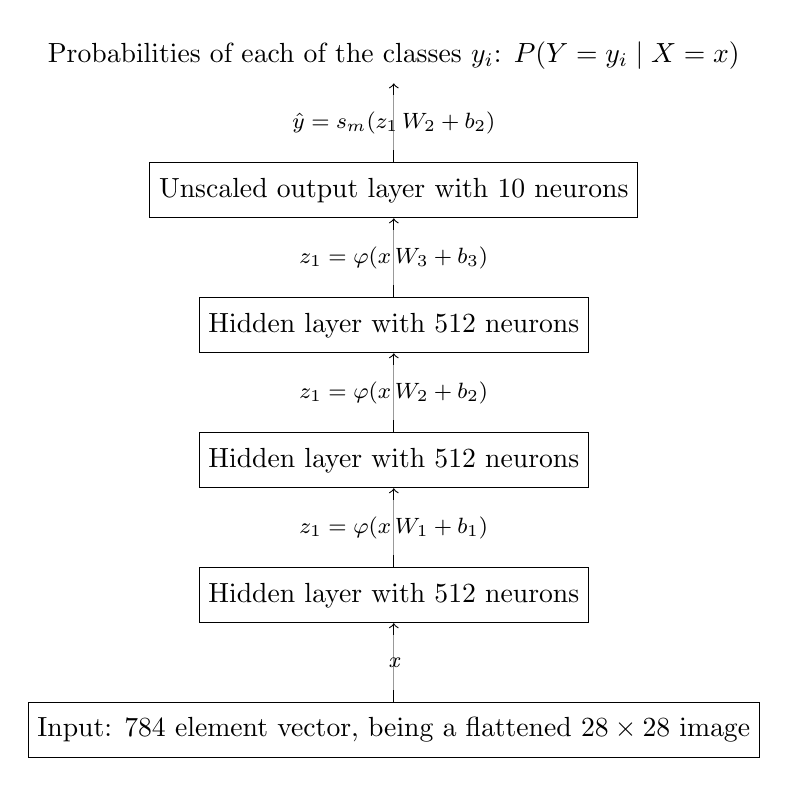
\begin{tikzpicture}[]

\node(in)[layer]{Input: 784 element vector, being a flattened $28 \times 28$ image};

\node(l1)[layer, above=of in]{Hidden layer with 512 neurons};
\node(l2)[layer, above=of l1]{Hidden layer with 512 neurons};
\node(l3)[layer, above=of l2]{Hidden layer with 512 neurons};

\node(lo)[layer, above=of l3]{Unscaled output layer with 10 neurons};
\node(out)[above=of lo]{Probabilities of each of the classes $y_i$: $P(Y = y_i \mid X=x)$};

\draw[->] (in) edge  node[labe]{x} (l1);
\draw[->] (l1) edge  node[labe]{$z_1=\varphi(x\,W_1+b_1)$} (l2);
\draw[->] (l2) edge  node[labe]{$z_1=\varphi(x\,W_2+b_2)$} (l3);
\draw[->] (l3) edge  node[labe]{$z_1=\varphi(x\,W_3+b_3)$} (lo);

\draw[->] (lo) edge  node[labe]{$\hat{y}=s_m(z_1\,W_2+b_2)$} (out);

\end{tikzpicture}

\end{document}